The first analysis we performed on the dataset we collected was to
understand how browser features have evolved over time. Understanding
and gaining insights into how Chrome and Firefox are dealing with new
as well as older features is important to be able to distill
conclusions about how secure and fingerprintable browsers are becoming
as they evolve. Hence, our analysis looked at specific browser
features that were introduced, what the typical lifespan of features
looks like.

After extracting feature information for all of the browsers under
analysis, we automatically parsed the generated reports and analyzed
them to see if the features in these browsers fall into specific
categories. Our analysis showed that the features in Firefox and
Chrome can be categorized in to three main categories:

\begin{itemize}
  
\item Persistent Features: These are features that are added to a
  specific version, and that continue to exist in every version that
  is released after the feature was introduced. We consider a feature
  to be ``persistent'' if it appears in at least two distinct browser
  versions.
      
\item Non-Persistent Features: These are features that existed in
  older versions of the browser, but were removed, and never appeared
  in newer version of the browser again. We consider a feature to be
  ``non-persistent'' if it is absent in at least two distinct versions
  of the browser under analysis.
      
\item Temporary Features: These are features that are added and
  removed from the browser from time to time. That is, they are
  introduced, they are removed, and they might appear again at some
  point. Such features are typically being tested by the vendors, and
  it is not clear if they will become persistent, or non-persistent.

\end{itemize}

Our analysis shows that Chrome possesses 9482 persistent, 711
non-persistent, and 3397 temporary features that it supports. In
contrast, Firefox supports 6237 persistent, 809 non-persistent, and
152 temporary features. Note that Firefox, overall, supports a less
number of features than Chrome. Also, our analysis shows that Firefox,
compared to Chrome, is keeping less features (i.e., they are removing
more) over time. Figures \ref{fig:chrome-categories} and
\ref{fig:firefox-categories} illustrate the feature categories for
each browser vendor.

\begin{figure}[ht]
    \centering
    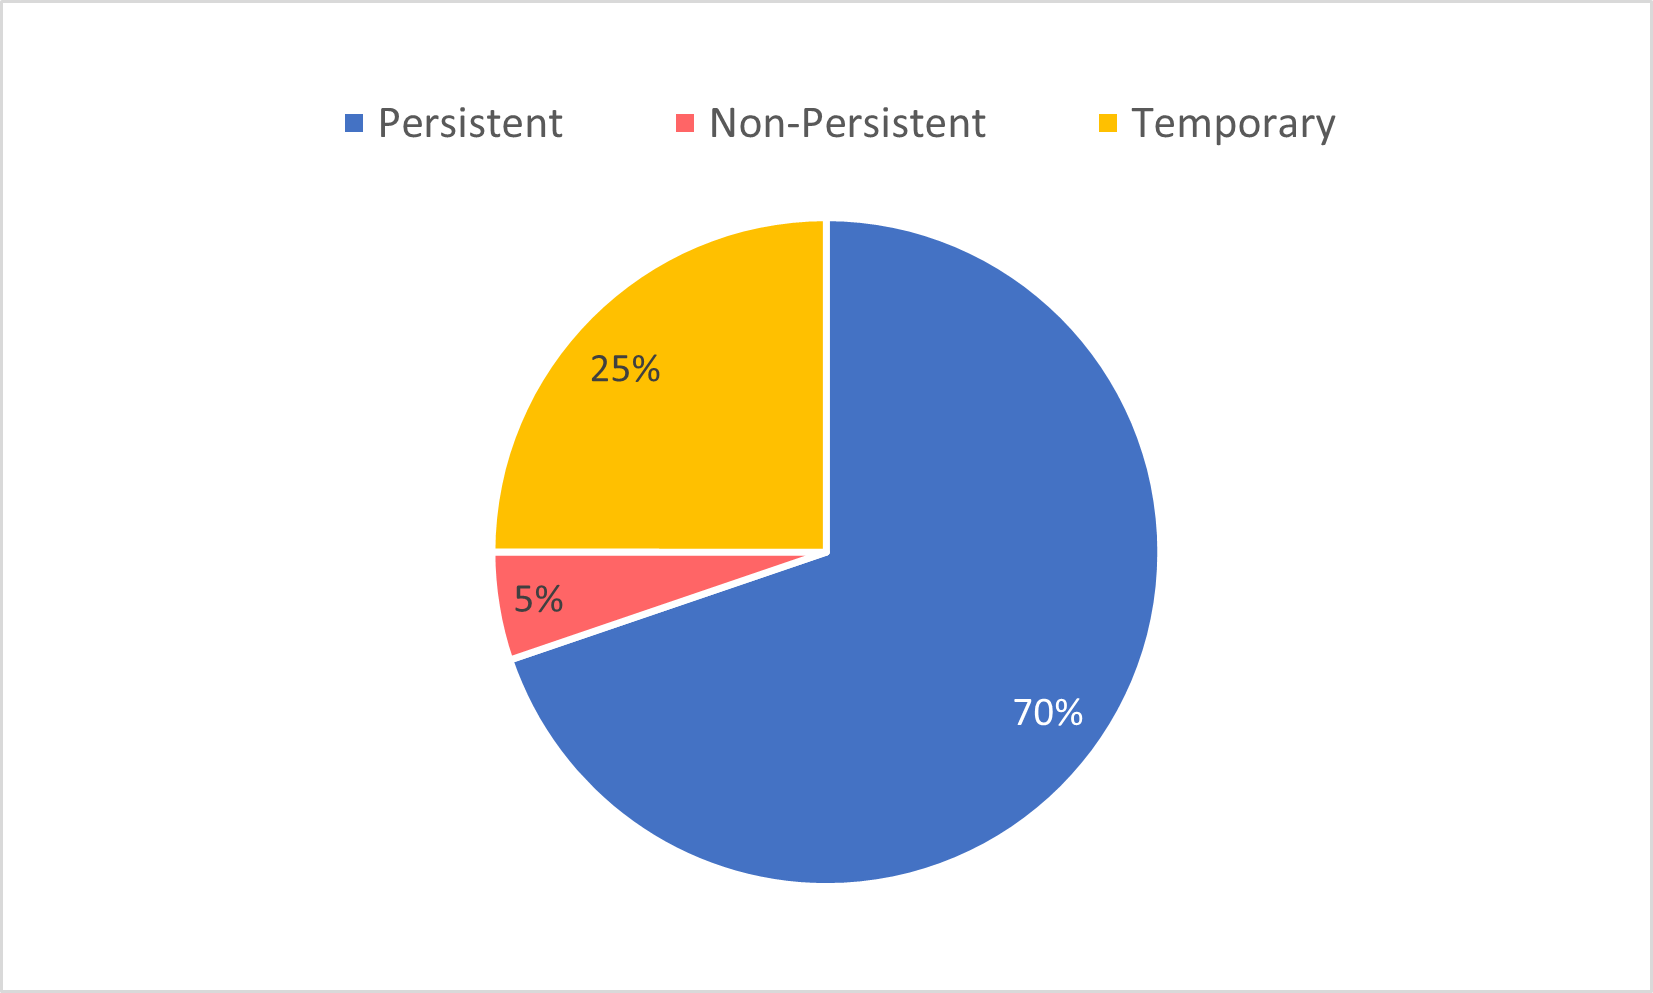
\includegraphics[width=\columnwidth]{figures/chrome-feature-categories.png}
    \caption{Feature category distribution for Chrome.}
    \label{fig:chrome-categories}
\end{figure}

\begin{figure}[ht]
    \centering
    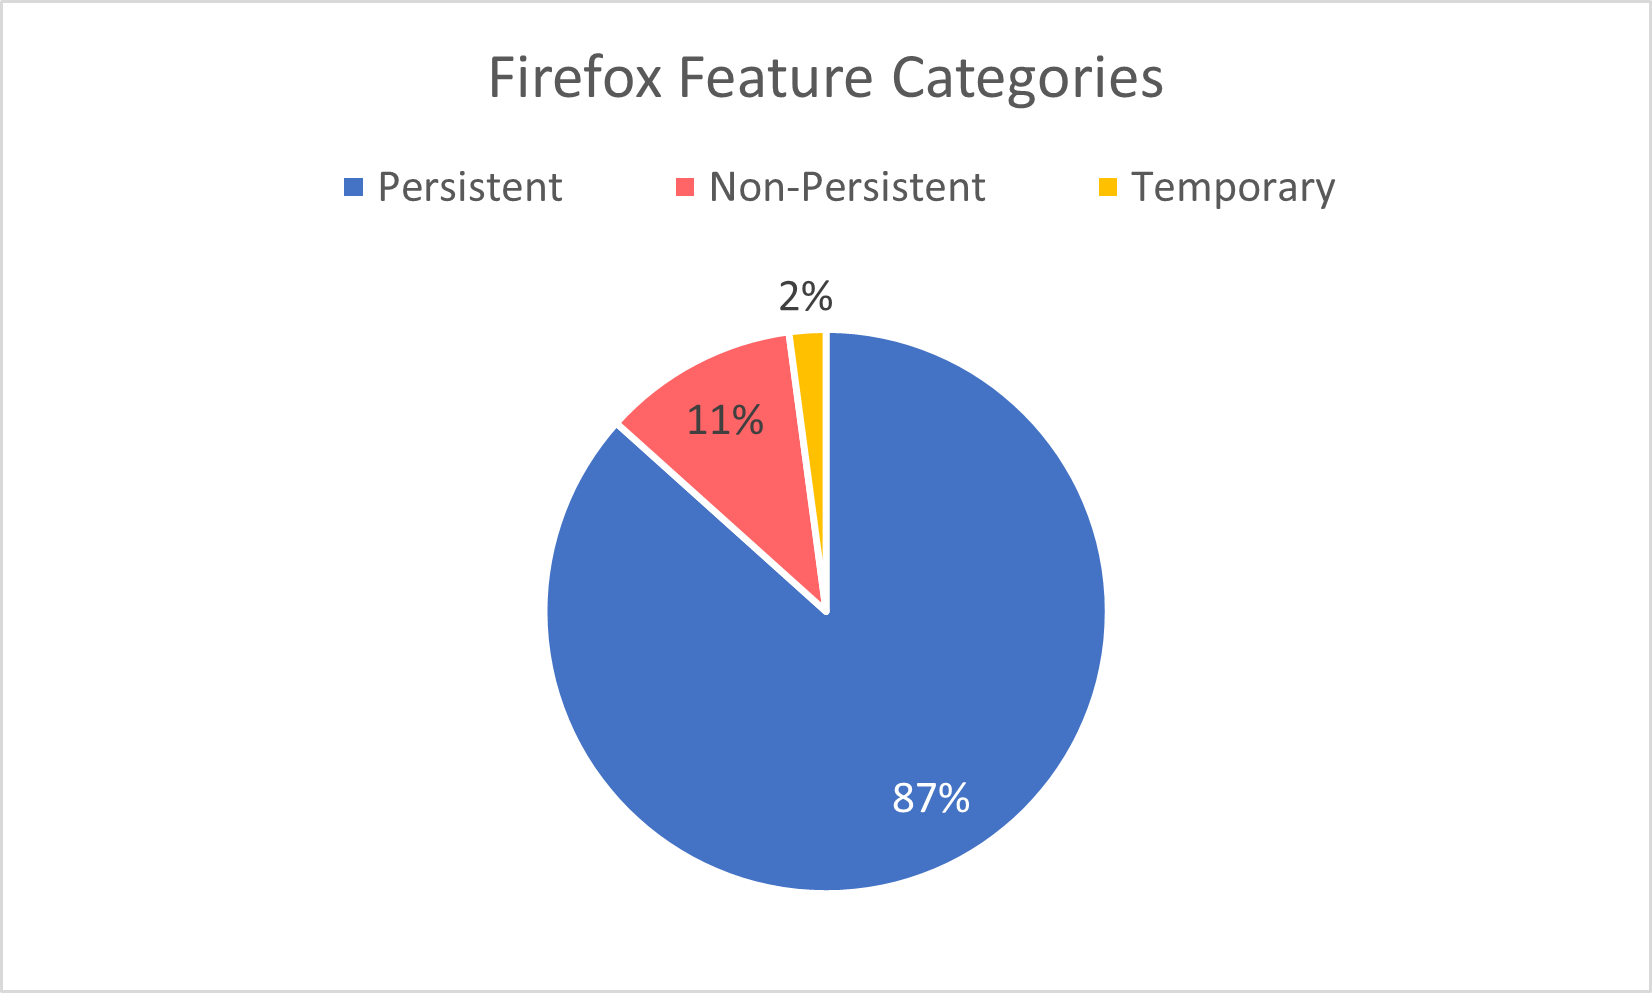
\includegraphics[width=\columnwidth]{figures/firefox-feature-categories.png}
    \caption{Feature category distribution for Firefox}
    \label{fig:times_bar}
  \end{figure}

  In this work, we also performed an analysis of the common features
  between Firefox and Chrome. Since 2016, the total number of features
  introduced by both Firefox and Chrome is 15,945. However, there
  exists only 4,843 common featur`es among them -- which is
  approximately \%30 of the total number of features that these
  vendors support. Hence, we can conclude that Firefox and Chrome do
  not have a high overlap of the features that they support. Note that
  although these browsers often offer very similar functionality,
  unsurprisingly, their code bases are very different and the APIs
  though which these features are available are also often
  significantly different. As a result, it is clear that
  vulnerabilities in these browsers will be very specific to the
  version and vendor.

  Figures \ref{fig:ffaddremove} and \ref{fig:chaddremove} show the
  feature addition and removal trends for Firefox and Chrome. The data
  shows that Chrome is adding and removing many more features than
  Firefox in each version that is released if one looks at the overall
  numbers of features. However, Firefox seems to be more constant with
  respect to the number of new features added, and older features
  removed.

\begin{figure}[ht]
    \centering
    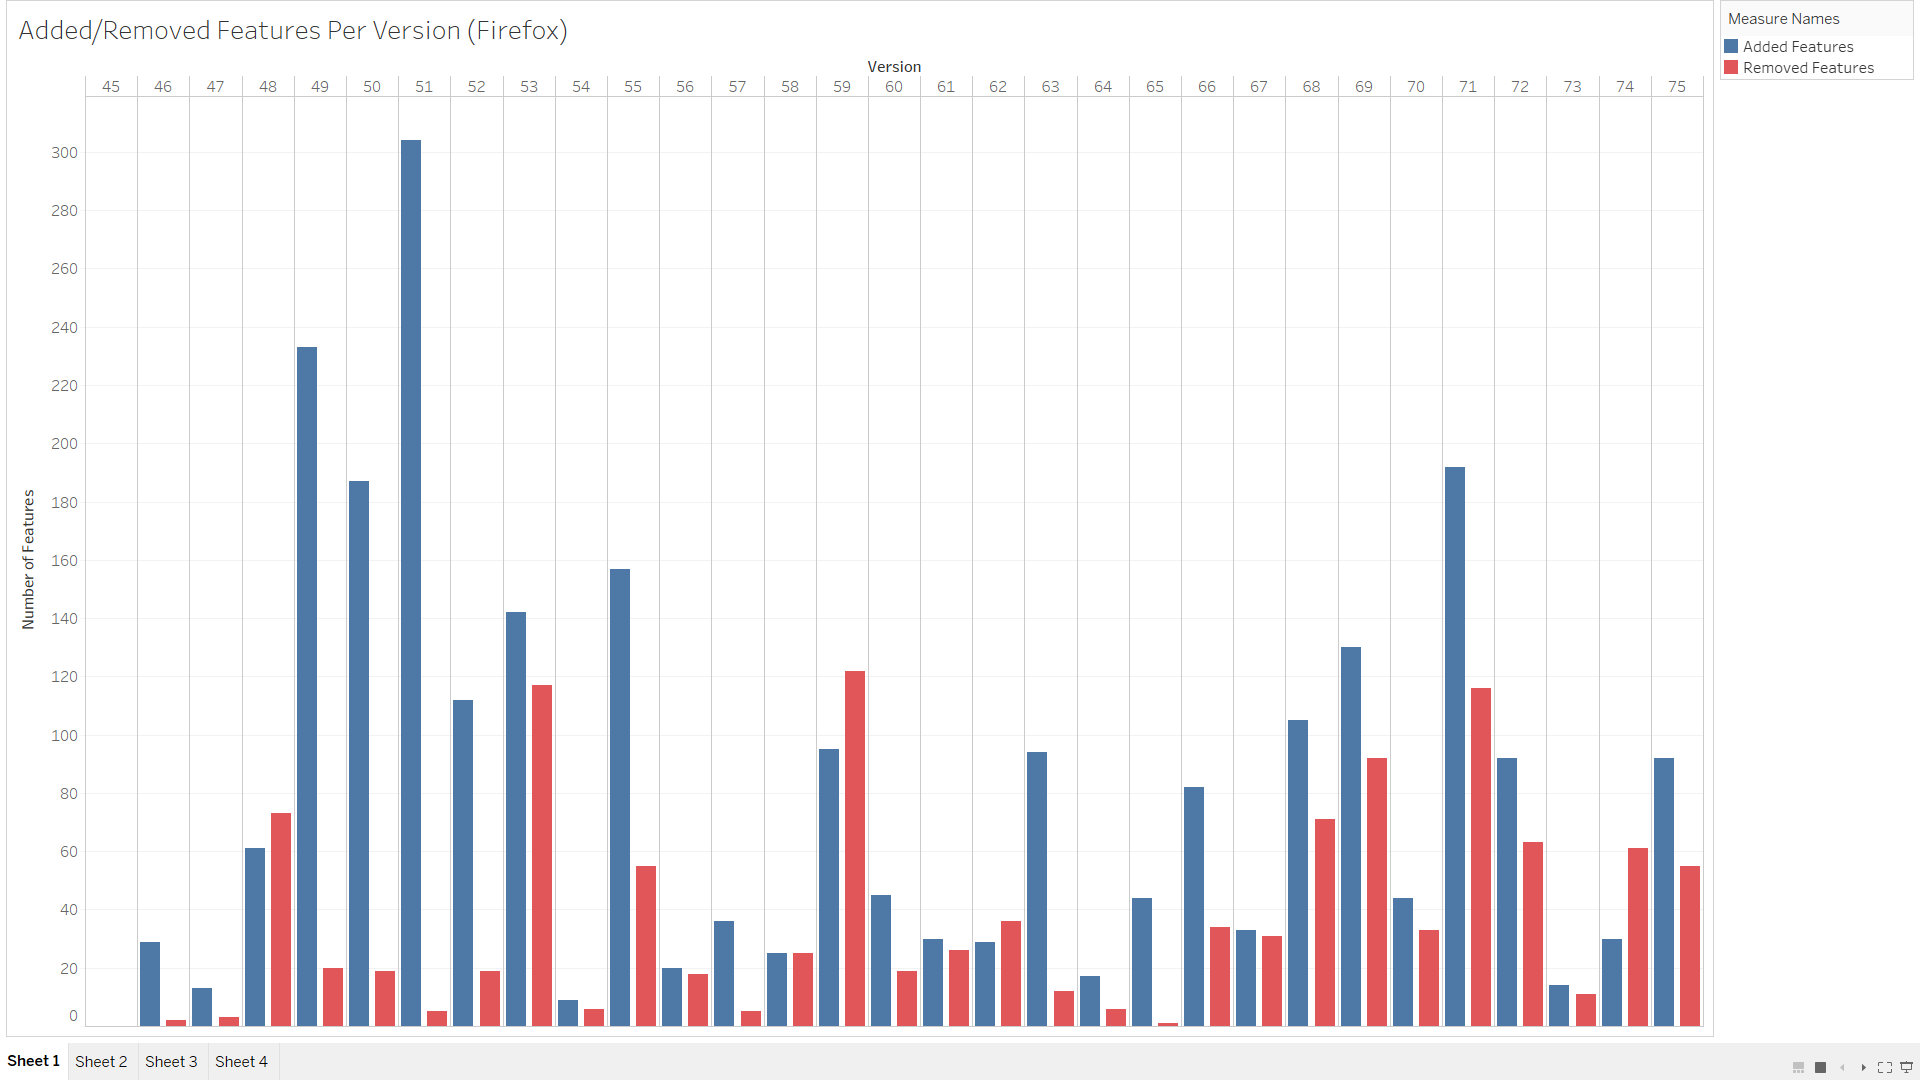
\includegraphics[width=\columnwidth]{figures/Firefox-add-remove.png}
    \caption{Feature introduction and removal in Firefox.}
    \label{fig:ffaddremove}
\end{figure}

\begin{figure}[ht]
    \centering
    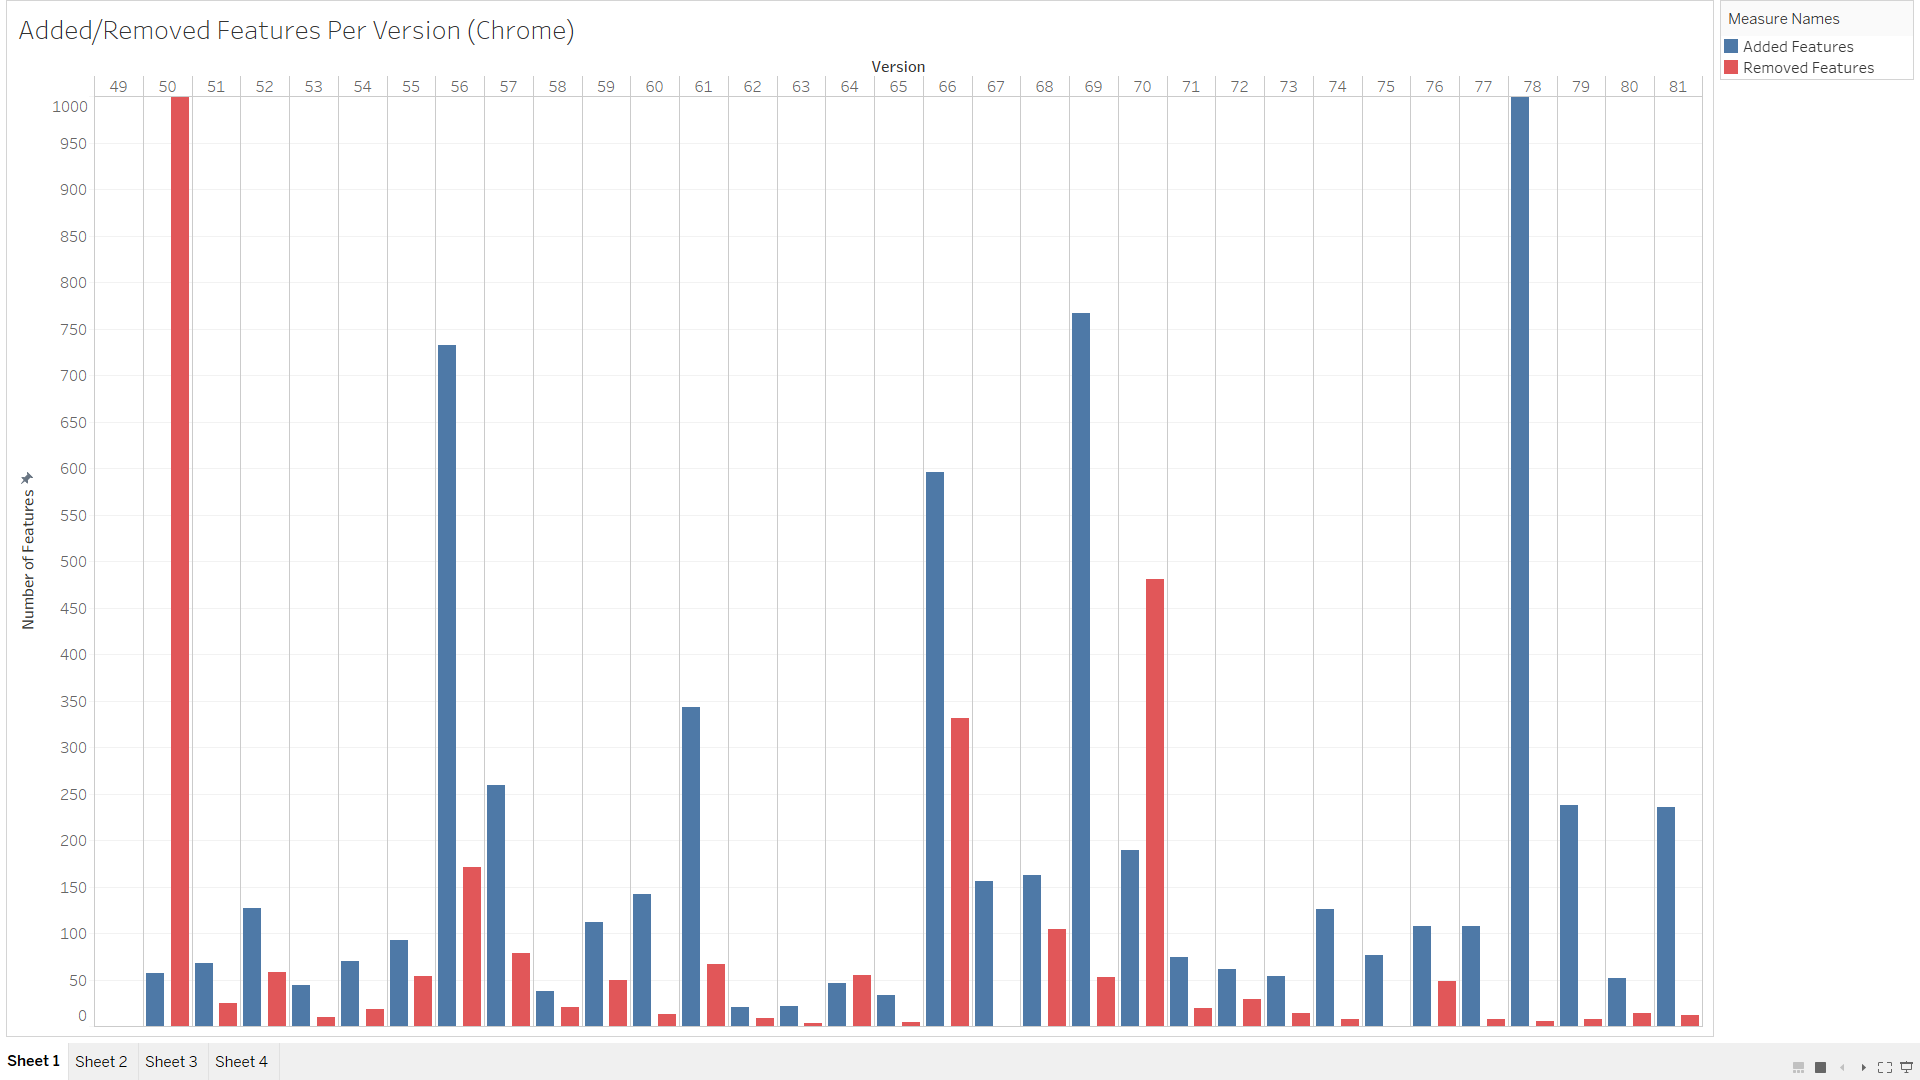
\includegraphics[width=\columnwidth]{figures/Chrome-add-remove.png}
    \caption{Feature introduction and removal in Chrome.}
    \label{fig:chaddremove}
\end{figure}

By using the feature datasets we extracted from the Firefox and Chrome
versions, we compared feature trends for both browsers. The trends are
depicted in Figure \ref{fig:featuretrends}. The graph shows that the
  number of features supported by Firefox seem to be quite steady
  (i.e., if new features are added, some older ones are typically
  removed) while the number of features supported by Chrome is growing
  over time. Hence, the data suggests that Chrome and Firefox are
  following differing browser feature development philosophies.

\begin{figure}[ht]
    \centering
    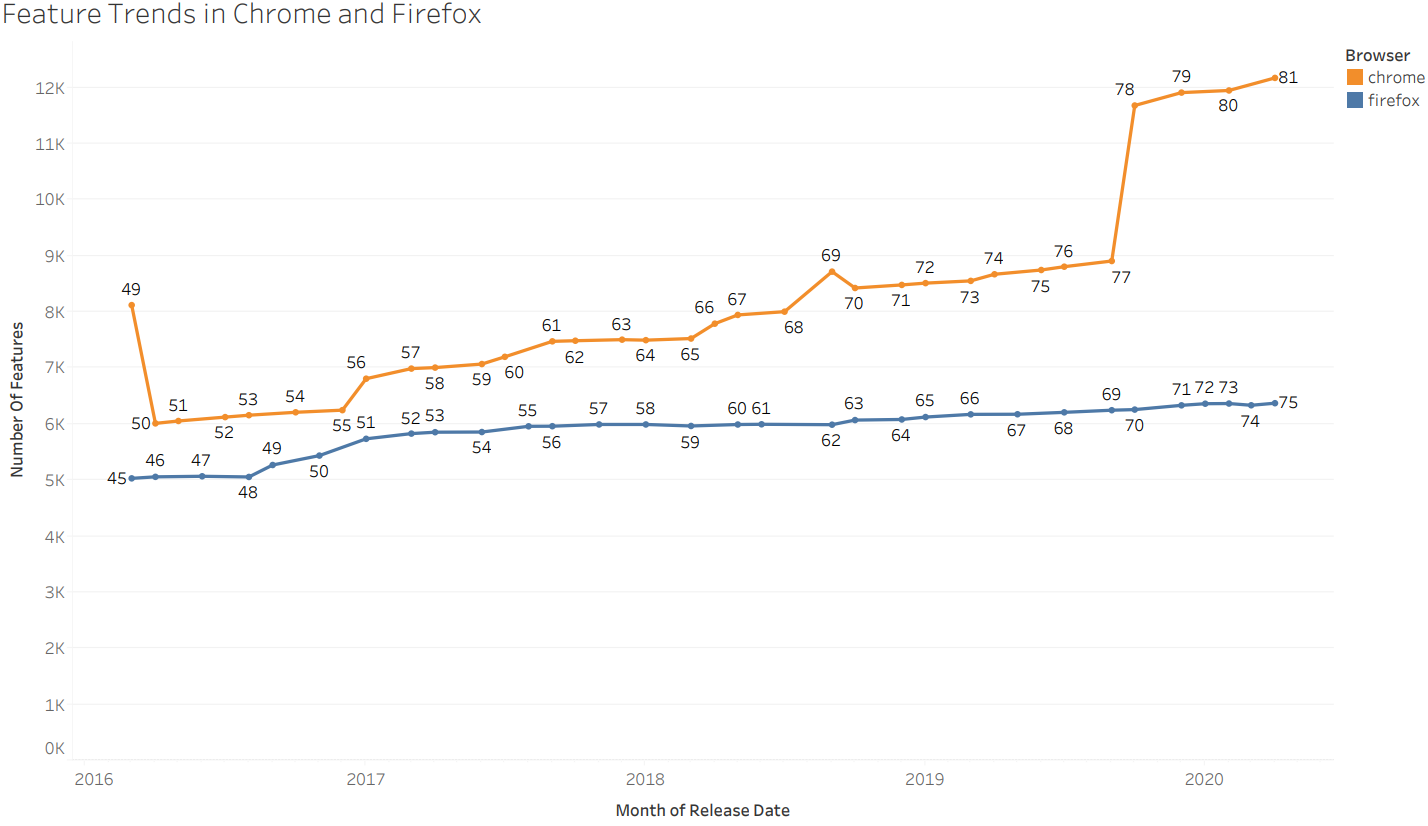
\includegraphics[width=\columnwidth]{figures/Feature-Trends.PNG}
    \caption{Feature trends in Firefox and Chrome when compared to
      each other.}
    \label{fig:featuretrends}
\end{figure}
